\section{Black Hole Fundamental Plane in Illustris}

\label{sec:analysis} To better understand the role of AGN in galaxy
evolution, we turn to large scale simulations with detailed gas physics
and energy transport like those found in the Illustris simulation.
To analyze the black hole feedback physics in the Illustris simulation,
we attempt to reconstruct the black hole fundamental plane from M03.
Starting with our sample of black holes from Section \ref{sec:sample},
we apply several models of a accretion mechanisms to parametrize the
components of the fundamental plane.

The fundamental plane from M03 is shown in Figure \ref{fig:Fp} and
defined as

\begin{equation}
\log L_{R}=0.6\log L_{x}+0.78\log M_{BH}+7.33
\end{equation}
where the $L_{R}$ is the radio luminosity, $L_{X}$ is the X-ray
luminosity, and $M_{BH}$ is the mass of the black hole. This expression,
derived from empirical observations of accreting black holes with
masses ranging from $10-10^{9}M_{\odot}$, correlates the energy output
from the black hole with its mass. Another way to parametrize the
fundamental plane is using the mass, accretion rate, and X-ray luminosity
which is given by

\begin{equation}
\log L_{x}=\log M+q\log\dot{M}+K\;\label{eq:LxFP}
\end{equation}
where $K$ is a normalization constant and $q$ reflects the efficiency
of the accretion mechanism. In M03, a range of $q$ values are given
from 0.5 (optically-thick thin disk) to 2.3 (advection dominated accretion
flow) depending on the assumed accretion physics.
\begin{figure}
\centering{}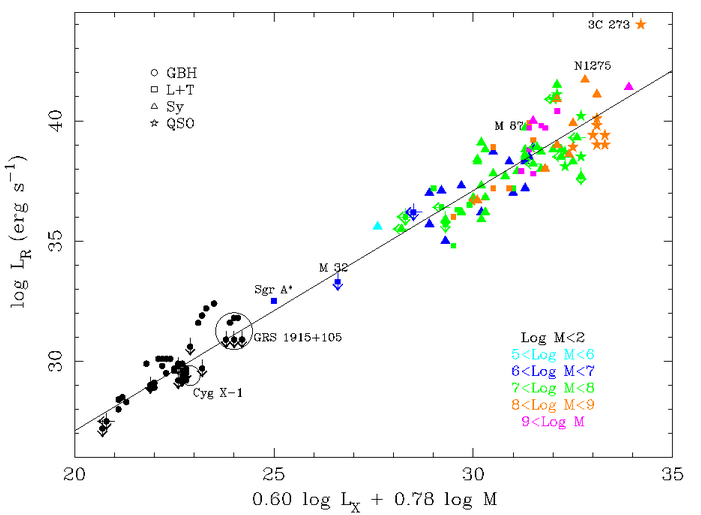
\includegraphics[clip,scale=0.35]{Figures/FP}\protect\caption{\label{fig:Fp}Edge-on view of the fundamental plane from M03 relating
the black hole mass to the radio and X-ray luminosities. Symbols indicate
the type of emission-line galaxy of the host and colors correspond
to the mass of the black hole in units of $\log\left({\rm M}_{\odot}\right)$.
Several well-known galaxies hosting an AGN are listed, as well.}
\end{figure}


The fundamental plane is expressed in terms of the X-ray luminosity
(Equation \ref{eq:LxFP}), but the Illustris simulation does not provide
any luminosities. We must therefore express the X-ray luminosity in
terms of those quantities provided by the simulation: black hole mass
and accretion rate. To accomplish this, we consider two models of
accretion. The first model is based on the Eddington luminosity and
assumes a spherically-symmetric and symmetrically-accreting mass surrounding
the black hole. Assuming that $10\%$ of the mass accreted onto the
black hole is converted into radiation, the bolometric luminosity
is given in column 1 of Table \ref{tab:luminosityConversions}. The
second model assumes an optically-thick, but physically thin, disk
of gas symmetrically accreting onto the black hole. Again assuming
an efficiency of $10\%$, the bolometric luminosity is given in column
1 of Table \ref{tab:luminosityConversions}.

Even for the most energetic black hole accretion, the X-ray luminosity
is only a fraction of the total light emitted the black hole. It therefore
stands to reason that there is a relation between the two luminosities
for a given black hole source. Using a set of 47 black holes from
the nearby universe, \citet{elvis1994atlasof} provide an empirical
correlation between the X-ray and bolometric luminosities (see Figure
\ref{fig:Elvis_template}). To convert the bolometric luminosities
from each of our assumed models into their respective X-ray luminosities,
we construct a power law fit to the Elvis data which has the form
\begin{figure}
\centering{}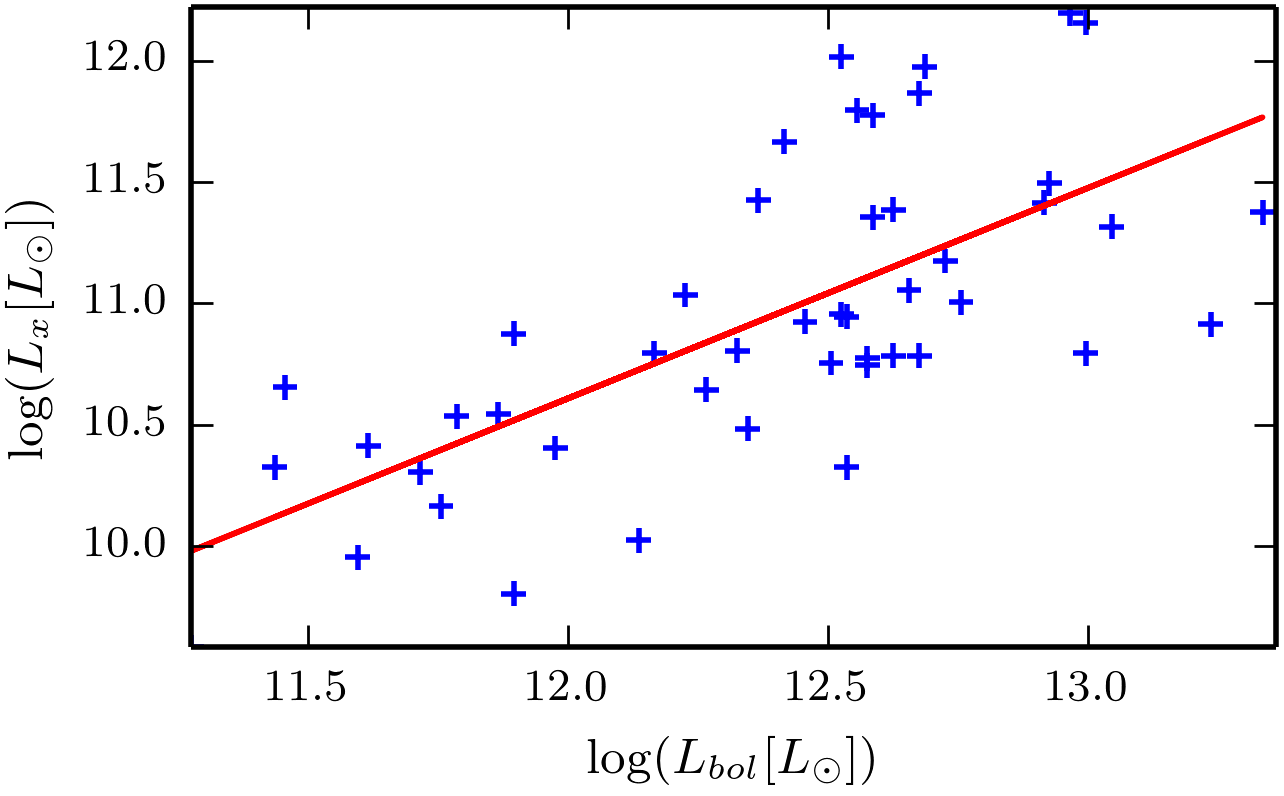
\includegraphics[clip]{Figures/elvis_template}\protect\caption{\label{fig:Elvis_template}Bolometric and X-ray luminosities from
the \citet{elvis1994atlasof} data set. The best-fit linear relation
is shown in red.}
\end{figure}


\begin{equation}
\log L_{x}=0.866\log L_{bol}+0.215\;.
\end{equation}
The conversion formulae between bolometric and X-ray luminosities
based on this power law are shown in Table \ref{tab:luminosityConversions}.
Combining these formulae with Equation \ref{eq:LxFP}, we can solve
the for both the efficiency parameter and the normalization constant.

Using the Levenberg-Marquard nonlinear least squares method, we find
a minimization in the black hole mass and mass accretion rate space
that gives the best fit to our desired parameters. For the first model
based on the Eddington luminosity approximation, we find $q=-0.0642\pm0.0005$
and $k=20.107\pm0.006$. For the second model based on the thin-disk
approximation, we find $q=0.379\pm0.0037$ and $k=4.99\pm0.0465$.
The physical interpretation of the efficiency parameter does not allow
for negative values. We therefore consider the Eddington model to
be inconsistent with the data from the Illustris simulation. For the
thin-disk model, our value of the efficiency parameter is within a
factor of $\sim2$ of the minimum value found by M03.
\begin{table}
\centering{}\protect\caption{\label{tab:luminosityConversions}}
\begin{tabular}{ccc}
\toprule 
Model & $L_{bol}$ & $L_{x}$\tabularnewline
\midrule
\midrule 
Eddington & $3.2\times10^{3}\, M_{BH}$ & $2.77\times10^{3}\, M_{BH}+0.215$\tabularnewline
\midrule 
Thin Disk & $4.648\times10^{19}\,\dot{M_{BH}}$ & $4.02\times10^{19}\,\dot{M_{BH}}+0.215$\tabularnewline
\bottomrule
\end{tabular}Bolometric (column 2) and X-ray (column 3) luminosity formulae for
the Eddington and think disk models. $M_{BH}$ is the mass of the
black hole in $M_{\odot}$ and $\dot{M}_{BH}$ is the accretion rate
in $M_{\odot}\: s^{-1}$.
\end{table}
\begin{figure}
\centering{}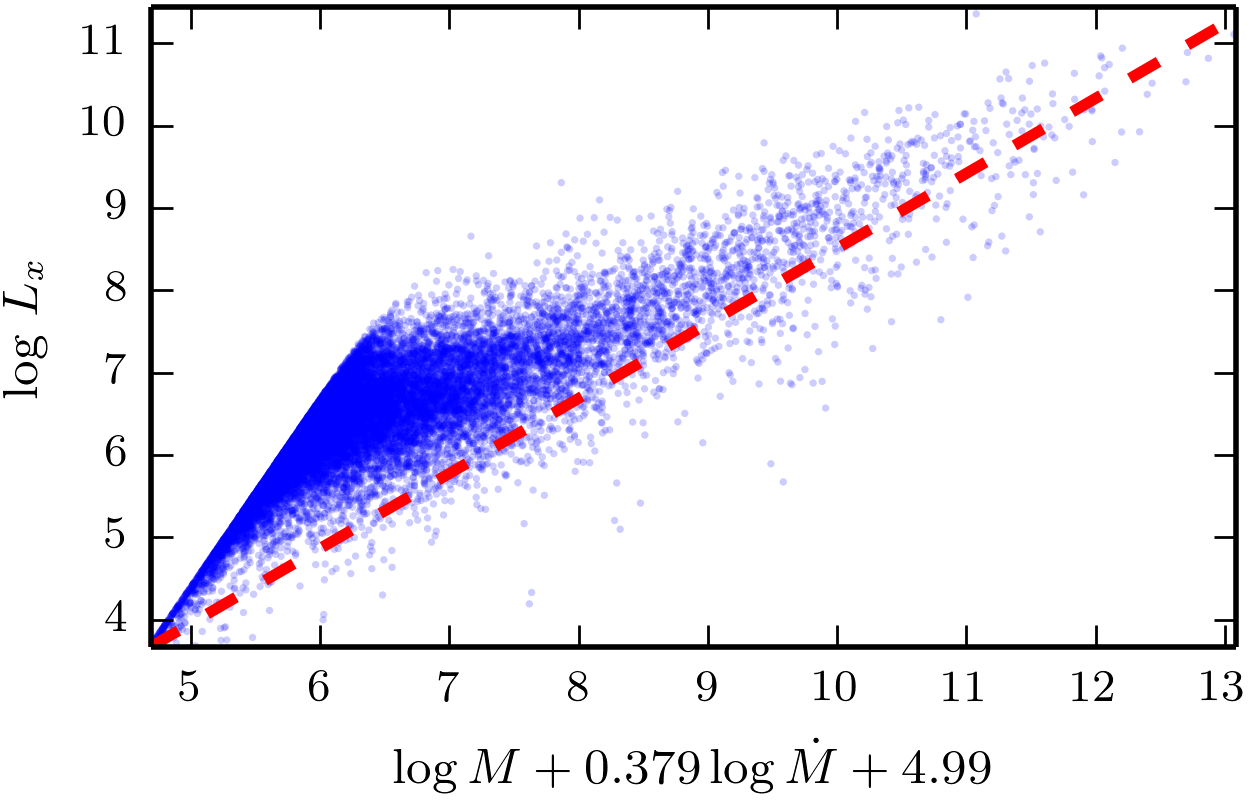
\includegraphics{Figures/fp_fit} \protect\caption{\label{fig:q_nr_hist}The fit to the fundamental plane $\log\left(L_{x}\,[L_{\odot}]\right)=\log M+0.378\log\dot{{M}}+9.47$
using our sample. The X-ray luminosities are in units of $L_{\odot}$,
the masses in units of $M_{\odot}$, and the accretion rate in units
of $M_{\odot}\, s^{-1}$.}
\end{figure}
